\input{../common}

\begin{document}
  %<*content>
  \lesson{analysis}{31}{Calcul intégral}
  

\subsection{Primitives d'une fonction numérique}
\begin{lemma}
Soit la fonction $ f : x \longmapsto 2x+3 $.

Calcule la dérivée de chacune des fonctions F ; G ; H définies par :

F$ (x)=x^{2} +3x+7$;  G$ (x)= x^{2} +3x-30$  et  H$ (x)=\paren{x+\frac{3}{2}}^{2} +10$. Que remarques-tu ?
\medskip

Pour tout $ x\in \mathscr{D}_f,\; $  F$' (x)=f(x),\;$  H$' (x)=f(x),\;$  G$' (x)=f(x)$.
\end{lemma}

\medskip
On dit que F ; G ; H sont  \textbf{des primitives de f sur Df}.

\begin{definition}
Soit $ f $ une fonction continue sur un intervalle $I$.

 On appelle fonction primitive de $f$ sur $I$ , toute fonction $F$ telle que :\\
$ \text{pour tout } \; x\in \text{I},\;  \text{F}'(x) = f (x).$
\end{definition}

\medskip


\begin{example}

Vérifions que la fonction : $\; F(x)=\dfrac{\eexp{2x}+1}{\eexp{x}+5}\; $  est une primitive sur $ \;\Rr\;  $ de la fonction $\; f\; $  définie sur $\; \Rr\; $  par: \\

 $  f(x)= \dfrac{\eexp{3x}+10\eexp{2x}-\eexp{x}}{(\eexp{x}+5)^{2}}$

\bigskip
Pour cela dérivons la fonction $F$.

\medskip
On a  $F'(x)=\dfrac{2\eexp{2x}(\eexp{x}+5)-\eexp{x}(\eexp{2x}+1)}{(\eexp{x}+5)^{2}}  =\dfrac{2\eexp{3x}+10\eexp{2x}-\eexp{3x}-\eexp{x}}{(\eexp{x}+5)^{2}}=\dfrac{\eexp{3x}+10\eexp{2x}-\eexp{x}}{(\eexp{x}+5)^{2}}$

Ainsi $F$ est une primitive de $ f. $
\end{example}



\begin{property}
 Si $F$ est une primitive de $ f $ sur I alors  toute  autre  fonction   de la  forme $ F(x)+c $ où $ c $ est une constante   est aussi primitive  de $ f $ sur I.
\end{property}

\medskip
\subsection*{Primitives des fonctions usuelles}

$$\begin{array}{|c|c|}
\hline
\textbf{Fonctions} \;f  &\textbf{ Primitives} \; F   \\ 
\hline
 a \; \text{un réel}  & ax \\
\hline
x^{n}    & \dfrac{x^{n+1}}{n+1} \\
\hline
 \dfrac{1}{\sqrt{x}}   &  2\sqrt{x}   \\
\hline
 \dfrac{1}{x}     &  \ln |x|     \\
\hline
\eexp{x}     &\eexp{x}    \\
\hline
\end{array}$$


\subsection*{Opérations sur les primitives}
\begin{property}
\noindent
Si F est une primitive de $f$ sur I et  G est une primitive de $g$ sur I alors:

\medskip
\noindent
$ \bullet $  F $+$ G est une primitive de $f + g$ sur I.

\medskip
\noindent
$ \bullet  $  Pour tout réel  $k$ ,\;  $k$F est une primitive de $kf$ sur I.
\end{property}
\medskip

Le tableau suivant découle des règles de dérivation des fonctions.

$ u $ désigne une fonction dérivable sur un intervalle I.


$$\begin{array}{|c|c|}
\hline
\textbf{Fonction}  &\textbf{ Primitive}     \\ 
\hline
 u'u^{n}   & \dfrac{u^{n+1}}{n+1}   \\
\hline
\dfrac{u'}{\sqrt{u}}    &  2\sqrt{u}    \\
\hline
\dfrac{u'}{u}  & \ln |u|      \\
\hline
u'\eexp{u}   &   \eexp{u}    \\
\hline
\dfrac{u'}{u^{n}}     &- \dfrac{1}{n-1} \dfrac{1}{u^{n-1}} \\
\hline

\end{array}$$



\medskip 
\begin{example}

Déterminons une primitive de chacune des fonctions suivantes.
\begin{enumerate}
\item $ f(x)= x^{2}-2x+5 $
\item  $ g(x)= 2x(x^{2}+3)^{2} $
\item $ h(x)=\eexp{x}(\eexp{x}+2)^{2} $

\item $ i(x)=\dfrac{2\eexp{x}}{\eexp{x}+1} $
\item $ j(x)=2+\dfrac{3}{(3x+4)^{2}} $
\item $ k(x)= x + 2-\dfrac{4}{2x-2}$
\end{enumerate}

\end{example}
\begin{proof}
\begin{enumerate}
\item  On a:\; F$(x)= \dfrac{1}{3}x^{3}-x^{2}+5x$
\item  $ g(x)= 2x(x^{2}+3)^{2} $  est de la forme  $f(x)= u'u^{n} $.

 Par suite  G$(x)= \dfrac{1}{3}(x^{2}+3)^{3} $.
\item $ h(x)=\eexp{x}(\eexp{x}+2)^{2} $ est de la forme  $f(x)= u'u^{n} $.                   

Par suite $ H(x)=\dfrac{1}{3}(\eexp{x}+2)^{3} $.
\item $ i(x)=\dfrac{2\eexp{x}}{\eexp{x}+1} $ est de la forme   $\dfrac{a u'}{u}$.


 Par suite   I$(x)=\ln (\eexp{x}+1) $.

\item $ j(x)=2+\dfrac{3}{(3x+4)^{2}} $  est   une somme de deux fonctions:  l'une étant une constante égale à $ 2 $  et l'autre de la forme $ \dfrac{ u'}{u^{2}}$.

Par conséquent  J$(x)=2x-\dfrac{1}{3x+4} $.

\item $ k(x)= x + 2-\dfrac{4}{2x-2}$\;  on fait la somme des deux primitives d'où:

K$(x)= \dfrac{1}{2}x^{2} + 2x-2\ln (2x-2)$
\end{enumerate}
 \end{proof}

\subsection{Intégrale d'une fonction}
\begin{definition}
Soit $ f $ une fonction continue sur un intervalle I et $  F $ une de ces primitives, soient $ a $ et $ b $ deux réels   de I.

Le nombre réel $ F(b)-F(a) $ est appelé intégrale de $ f $ entre $ a $ et $ b $ et est notée   $\; \inte{a}{b}{f(x)}{x} $. 
\\ Ainsi on a:
$$ \inte{a}{b}{f(x)}{x} =F(b)-F(a) $$

\end{definition}

 \textbf{Vocabulaire  et notations}
 \begin{itemize}
 \item Le réel  $\; \inte{a}{b}{f(x)}{x}\;  $ \; se lit  <<  intégrale  de $a$  à $b$  \;f$(x)\; dx$  >>
 \item Le nombre $a$ est appelé borne inférieure et $b$ la borne supérieure de l'intégrale
\item Pour toute primitive F de f, on écrit \;   $ \inte{a}{b}{f(x)}{x}=\croch {F(x)}^{b}_{a} =F(b)-F(a) $.\\
L'expression \;$ \croch {F(x)}^{b}_{a} $\; se lit <<  $ F(x) $>>  pris entre a et b.
\item  Dans l'écriture  $ \inte{a}{b}{f(x)}{x} $, on peut remplacer la lettre $ x $ par n'importe quelle    lettre  et on peut écrire   $ \;\inte{a}{b}{f(x)}{x}  =  \inte{a}{b}{f(u)}{u} =  \inte{a}{b}{f(t)}{t} $.\; On dit que $ x $ est une variable muette,  elle n'intervient pas dans le résultat.
  \end{itemize}
  
  \medskip
  \begin{example}
  
Calculons $\;  \inte{0}{1}{(x^{2}-1)}{x} \quad$   et  \quad$\inte{-1}{0}{\eexp{-2x}}{x}  $.
 
  \bigskip
$ \bullet \; $   Une primitive de la fonction  $ x\longmapsto x^{2}-1 \; $  sur $\;  \intff{0}{1} $ est la fonction  F: $ x\longmapsto \frac{1}{3}x^{3}-x $\\ On a donc  $\;  \inte{0}{1}{(x^{2}-1)}{x}= \croch{\frac{1}{3}x^{3}- x}^{1}_{0}=F(1)-F(0) =-\frac{2}{3}$.

\medskip

$ \bullet \; $   Une primitive de la fonction  $ x\longmapsto \eexp{-2x}$  sur $ \Rr $ est la fonction  G: $ x\longmapsto  \frac{-\eexp{-2x}}{2} $\\


On a donc  $\;  \inte{-1}{0}{\eexp{-2x}}{x}=G(0)-G(-1)= \frac{\eexp{2} -1}{2}$
\end{example}
 

  \subsection*{Propriétés  de l'intégrale}
  \begin{property}
 Soit $f$  et $g$ deux fonctions continues sur un intervalle I contenant les réels  $a $, $b  $  et $c $. Alors:     
 \begin{itemize}
  \item[$  \bullet$]  $ \inte{a}{a}{f(x)}{x} =0$ 
  \item[$  \bullet$] $ \inte{a}{b}{f(x)}{x} = -\inte{b}{a}{f(x)}{x}$
  \item[$  \bullet$] $ \inte{a}{c}{f(x)}{x} +\inte{c}{b}{f(x)}{x}=\inte{a}{b}{f(x)}{x}$\;
  
  (Relation de Chasles)
\item[$  \bullet$]   $ \inte{a}{b}{\alpha f(x)}{x} =\alpha\inte{a}{b}{f(x)}{x}$;\; $\alpha\in\Rr$.
   \item[$  \bullet$] $ \inte{a}{b}{f(x)}{x} +\inte{a}{b}{g(x)}{x}=\inte{a}{b}{f(x)+g(x)}{x}$
 
\end{itemize}


 \end{property}
 

 
 \subsection{Calculs d'aires}

Le plan est muni d'un repère orthogonal  $ \oij $. \\ L'unité d'aire notée par \textbf{u.a},\;  est l'aire du rectangle de dimensions     $ ||\overrightarrow{i}|| $  et   $ ||\overrightarrow{j}|| $.

\begin{tikzpicture}
\draw[thick,black,dashed] (-1,0)  (2,2);
\draw[thick] (-1,0) -- (2,0);
\draw [thick](0,0) -- (0,2);
\draw[thick,red,->,>=stealth'] (0,0) -- (0.5,0) node[midway,below] {$\overrightarrow{i}$};
\draw[thick,red,->,>=stealth'] (0,0) -- (0,1) node[midway,left] {$\overrightarrow{j}$};
\node[below left] at (0,0) { O};
\clip (-1,0) rectangle (2,2);
\draw[thick,black,dashed] (0.5,1) -- (0.5,0);
\draw[thick,black,dashed] (0.5,1) -- (0,1);
\end{tikzpicture}


 
 \begin{definition}
 

 Le  plan est  muni d'un repère orthogonal.\\ Soit $f$ une fonction continue et\textbf{ positive} sur un intervalle $ \intff{a}{b} $  et  $F$ une primitive de $f$ sur $ \intff{a}{b} $.\\

  L'aire ( en u.a) de la partie du plan délimitée par la courbe de $f$, l'axe des abscisses et les droites d'équations $\; x=a\;$ et $ \;x=b$, est égale à l'intégrale  $\; \inte{a}{b}{f(x)}{x} $.
\end{definition}
\begin{center}
\begin{tikzpicture}[scale=0.8]
\draw[gray!25] (-4,-1) grid (3,3);
\fill[bottom color=blue!25,top color=blue!35!black,opacity=0.5] (-3,0)  plot[domain=-3:2,samples=100] (\x,{0.125*\x*\x*\x+0.125*\x*\x-\x+1}) -- (2,0) -- (-3,0);
\draw[thick,->,>=stealth'] (-4,0) -- (3,0);
\draw[thick,->,>=stealth'] (0,-1) -- (0,3);
\foreach\x in {}
{
	\draw[thick] (\x,0.1) -- (\x,-0.1) node[below] {\tiny\x};
}
\foreach\y in {}
{
	\draw[thick] (-.1,\y) -- (0.1,\y) node[right] {\tiny\y};
}
\node[below left] at (0,0) {\tiny O};
\draw[thick,blue!50!black] plot[domain=-4:3,samples=100] (\x,{0.125*\x*\x*\x+0.125*\x*\x-\x+1}) node[right] {$\mathscr{C}_f$};
\draw[very thick,blue!50!black] plot[domain=-3:2,samples=100] (\x,{0.125*\x*\x*\x+0.125*\x*\x-\x+1});
\node[white] at (-1.5,1) {$ \inte{a}{b}{f(x)}{x}$};
\node  at (-3,-0.5) {$ a $};
\node  at (2,-0.5) {$ b $};
\end{tikzpicture}
\end{center}

\begin{remark}

Lorsque $ f $ une fonction continue et\textbf{ négative} sur un intervalle $\; \intff{a}{b} $.\\
 L'aire ( en u.a) de la partie du plan délimitée par la courbe de $f$, l'axe des abscisses et les droites d'équations $ x=a$ et $ x=b$, est égale à l'intégrale  $ \;-\inte{a}{b}{f(x)}{x} $.
\end{remark}

\medskip

\begin{exercice}

Soit  la fonction $ f $  définie sur  $ \Rr $  par $ f(x)=x^{3}-3x $.\\
Etudier les variations de $ f $ et construire sa courbe dans un repère  orthonormé d'unité 2 cm.\\
En déduire l'aire en cm$ ^{2} $ de la partie comprise entre les
droites d'équation $x = 0$ et $x = \sqrt{3}$, l'axe des abscisses
et la courbe représentative de $ f$.
\end{exercice}

\begin{proof}
$ f $ est une fonction dérivable sur $ \Rr $  et $ f'(x)=3x^{2}-3=3(x-1)(x+1) $.  D'où le tableau de variation suivant.

\begin{tikzpicture}[scale=0.6]
\tkzTab[lgt=1.5]
{
	$x$ / 1 ,
	$f^{\prime}(x)$ / 1,
	$f(x)$ / 2
}
{ $-\infty$ , $-1$ , $1$ , $+\infty$ }
{ , + , z , - , z , + , }
{ -/$-\infty$ ,  +/$2$, -/$-2$ , +/$+\infty$ }
\end{tikzpicture}

\begin{tikzpicture}[scale=0.8]
\draw[gray!25] (-4,-1) grid (3,3);
%\fill[bottom color=blue!25,top color=blue!35!black,opacity=0.5] (-3,0)  plot[domain=-3:2,samples=100] (\x,{0.125*\x*\x*\x+0.125*\x*\x-\x+1}) -- (2,0) -- (-3,0);
\draw[thick,->,>=stealth'] (-3,0) -- (3,0);
\draw[thick,->,>=stealth'] (0,-2) -- (0,2);
\foreach\x in {}
{
	\draw[thick] (\x,0.1) -- (\x,-0.1) node[below] {\tiny\x};
}
\foreach\y in {}
{
	\draw[thick] (-.1,\y) -- (0.1,\y) node[right] {\tiny\y};
}
\node[below left] at (0,0) { O};
\draw[thick,blue!50!black] plot[domain=-1.9:2,samples=50] (\x,{\x*\x*\x-3*\x}) node[right] {$\mathscr{C}_f$};
%\draw[very thick,blue!50!black] plot[domain=-3:2,samples=100] (\x,%{0.125*\x*\x*\x+0.125*\x*\x-\x+1});
%\node[white] at (-1.5,1) {$\pmb{ \inte{a}{b}{f(x)}{x}}$};
%\node  at (-3,-0.5) {$ a $};
\node  at (2,-0.5) {$ \sqrt{3} $};
\end{tikzpicture}


Sur l'intervalle $ \intff{0}{\sqrt{3}} $  la fonction $ f $  est continue et négative  et a pour primitive $ F(x)=\dfrac{1}{4}x^{4}-\dfrac{3}{2}x^{2}$.

Une unité d'aire est égale à 4 cm$ ^{2} $.

L'aire de la partie en question est égale à:

$\mathcal{A}=-\inte{0}{\sqrt{3}}{f(x)}{x} = -\inte{0}{\sqrt{3}}{(x^{3}-3x)}{x}=-(F(\sqrt{3})-F(0))=2.25$

Soit  en unité d'aire  $\mathcal{A}= 2.25\times 4 cm^{2}=9 cm^{2} $
\end{proof}

 
 \end{document}  